%\pagenumbering{arabic}%start arabic pagination from 1 

\chapter{Praktická část}

popis

\section{Návrh}

Schéma myšlenkové mapy.

\begin{lstlisting}
{
	"_id": "1234-5678-9012-3456",
	"name": "Berries",
	"children": [
		{
			"key": "1",
			"name": "Grapes",
			"children": [
				{
					"key": "2",
					"name": "Red grapes"
				},
				{
					"key": "3",
					"name": "Green grapes"
				}
			]
		},
		{
			"key": "4",
			"name": "Strawberries"
		},
		{
			"key": "5",
			"name": "Blueberries"
		}
	]
}

\end{lstlisting}

\subsection{Cíle aplikace}

\begin{itemize}
\item Přidání a odstranění myšlenkových map
\item Přidání a odstranění jednotlivých bodů v myšlenkové mapě
\item Nevim
\end{itemize}

\subsection{Architektura}



\section{Řídící verticle}

Vzhledem k tomu, že bude aplikace nasazená na více serverech ve více rolích bylo by potřeba napsat několik modulů podle zaměření, které tam startovat. To lze vyřešit napsáním ,,startéru", který dle konfigurace nastartuje příslušné moduly či verticly.

\begin{lstlisting}
JsonObject config = new JsonObject();
config.putString("foo", "wibble");
config.putBoolean("bar", false);
container.deployVerticle("foo.ChildVerticle", config);
\end{lstlisting}

Spuštění verticle z příkazové řádky
\begin{lstlisting}
vertx run foo.js -conf myconf.json
\end{lstlisting}

\section{Integrace s databází MongoDB}

databaze

\section{Komunikace v reálném čase}\label{sec:realTimeCommunication}

Po načtení myšlenkové mapy přichází na řadu aspekty komunikace v reálném čase. V rámci editoru myšlenkových map budou implementovány tři základní operace.
\begin{itemize}
\item Přidání objektu do myšlenkové mapy
\item Odstranění objektu z myšlenkové mapy
\item Přejmenování objektu v myšlenkové mapě
\end{itemize}
V tradiční webové aplikaci by to znamenalo implementaci těchto metod typem požadavek-odpověď jako operací konkrétní API. Při přidání objektu by se zavolala API a nazpět by přišla odpověď zda-li byla akce úspěšná. Pokud bychom však chtěli mít editor, který by propagoval změny ke všem, kdo mají myšlenkovou mapu otevřenou museli bychom znát přihlášené uživatele, kterým by server poslal notifikaci o změně. Mnohem jednoduší cesta je rozdělení požadavku a odpovědi do dvou částí což odpovídá návrhovému vzoru Command. V takovém případě při otevření webového prohlížeče s danou myšlenkovou mapou dojde k zaregistrování klienta na určitou adresu. V případě jakékoli změny, kterou provede jiný uživatel nebo kdokoliv jiný, dojde k odeslání události všem zaregistrovaným klientům okamžitě v době vykonání události. Tuto situaci lze vidět na obrázku \ref{fig:realtime_communication}. V případě, kdy u uživatele dojde k vyvolání akce, ostatním uživatelům bude zaslána událost, která s sebou nese všechny informace o změně. Všem klientům zaregistrovaným na stejnou adresu přijde stejná událost. Tento typ zasílání zpráv je znám jako návrhový vzor Publish/Subscribe.

\begin{figure}
\begin{centering}
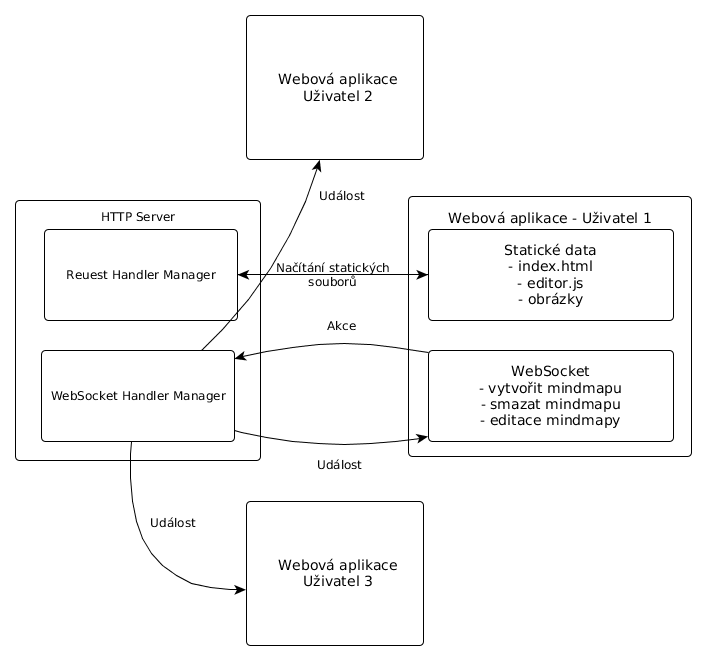
\includegraphics[width	=1\textwidth]{obrazky/realtime_communication}
\par\end{centering}
\caption{Komunikace v reálném čase\label{fig:realtime_communication}}
\end{figure}

\subsection{Akce}

Když bude uživatel chtít změnit myšlenkovou mapu (přidat objekt, odebrat objekt nebo přejmenovat objekt), vyšle akci na server. Tato akce bude poslána přes přemostěný event bus, který byl představen v kapitole \ref{sub:eventBus}. Na straně serveru je pak verticle, který má zaregistrovány metody na příchozí akce. Samotná akce nemá žádnou návratovou hodnotu, pokud tak dojde k chybě nedojde k vyslání události, která s sebou nese změny myšlenkové mapy.

\subsection{Události}

Pokud uživatel otevře webový prohlížeč s konkrétní myšlenkovou mapou, dojde tak k přihlášení odběru událostí nad touto myšlenkovou mapou. Pokud ji někdo změní tento uživatel dostane stejnou událost s informací o změně jako každý jiný uživatel přihlášený k odběru událostí.
Na straně klienta tak budou implementovány metody, které budou mít definované chování pro každou z definovaných událostí: přidání, odebrání a přejmenování objektu v myšlenkové mapě.

\section{Polyglot vývoj a moduly}\label{sec:praktickyModuly}

 deskriptor\emph{toto je poze základní výčet parametrů všechny lze nalézt v dokumentaci Vert.x}

\begin{lstlisting}
{
  "main": "EchoServer.java",
  "worker": true,
  "includes": "io.vertx~some-module~1.1",
  "auto-redeploy": true
}
\end{lstlisting}

\begin{figure}
\begin{centering}
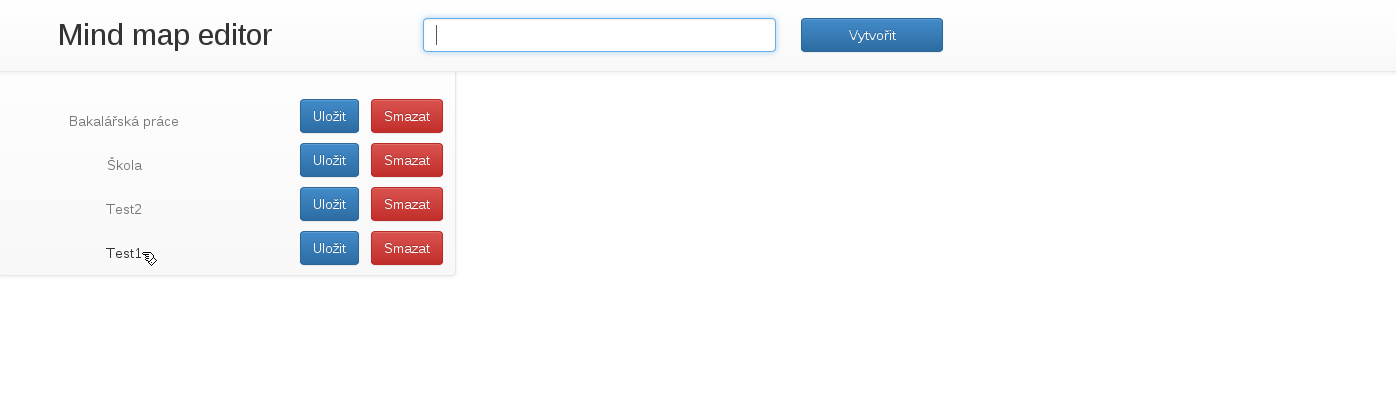
\includegraphics[width	=1\textwidth]{obrazky/mindmap1}
\par\end{centering}
\caption{Webová aplikace\label{fig:midnmap1}}
\end{figure}

\begin{figure}
\begin{centering}
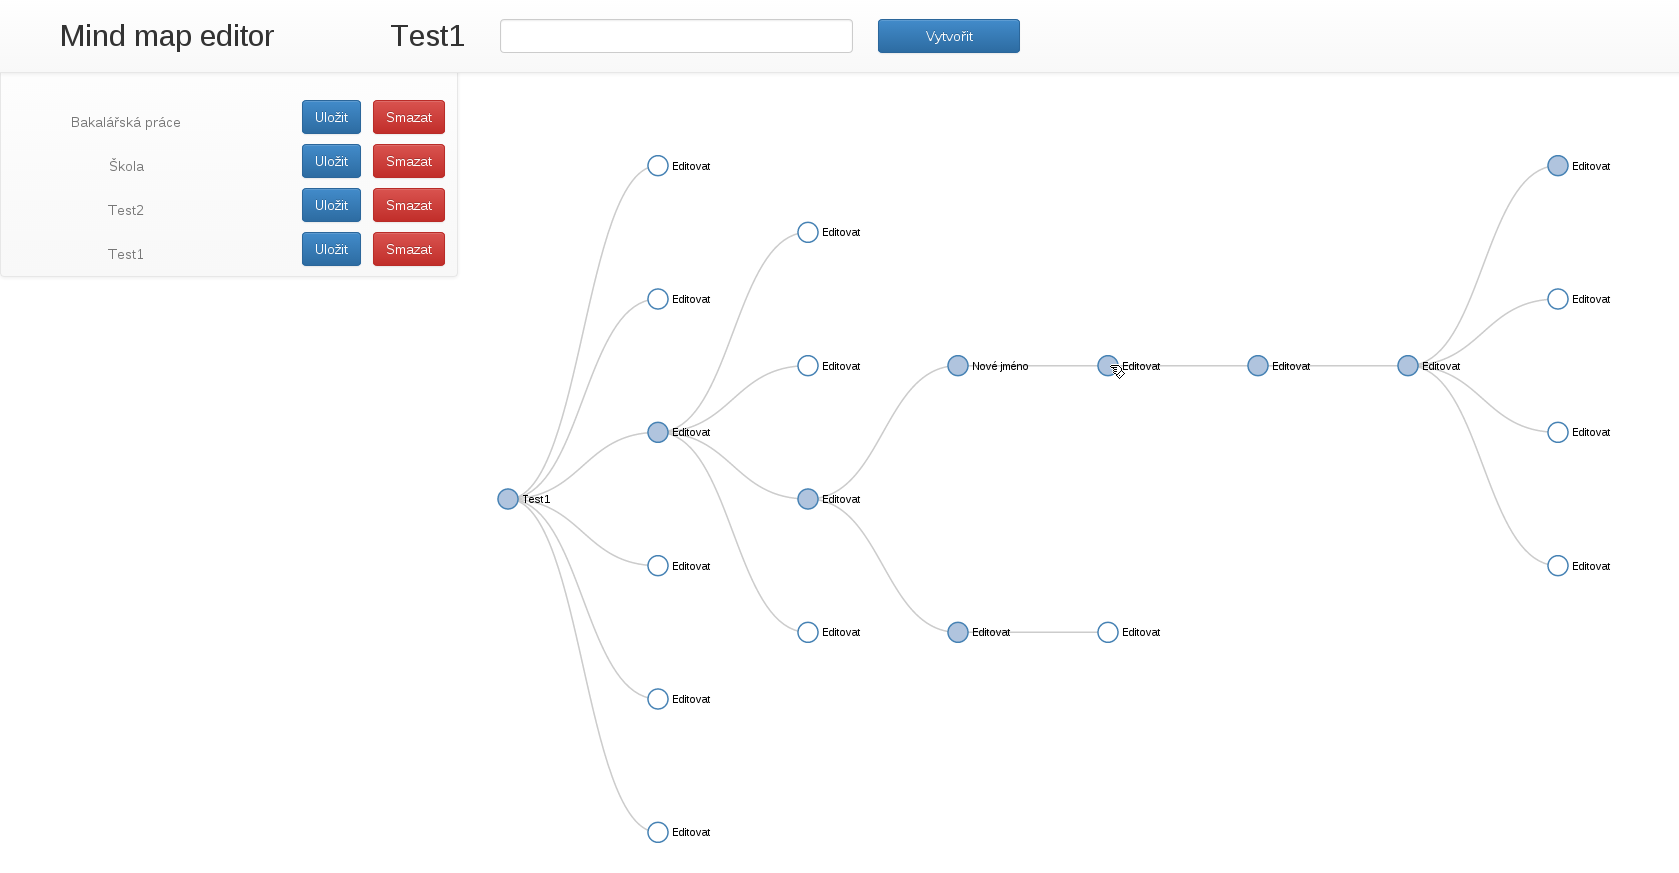
\includegraphics[width	=1\textwidth]{obrazky/mindmap2}
\par\end{centering}
\caption{Webová aplikace - otevření myšlenkové mapy\label{fig:midnmap2}}
\end{figure}

\begin{figure}
\begin{centering}
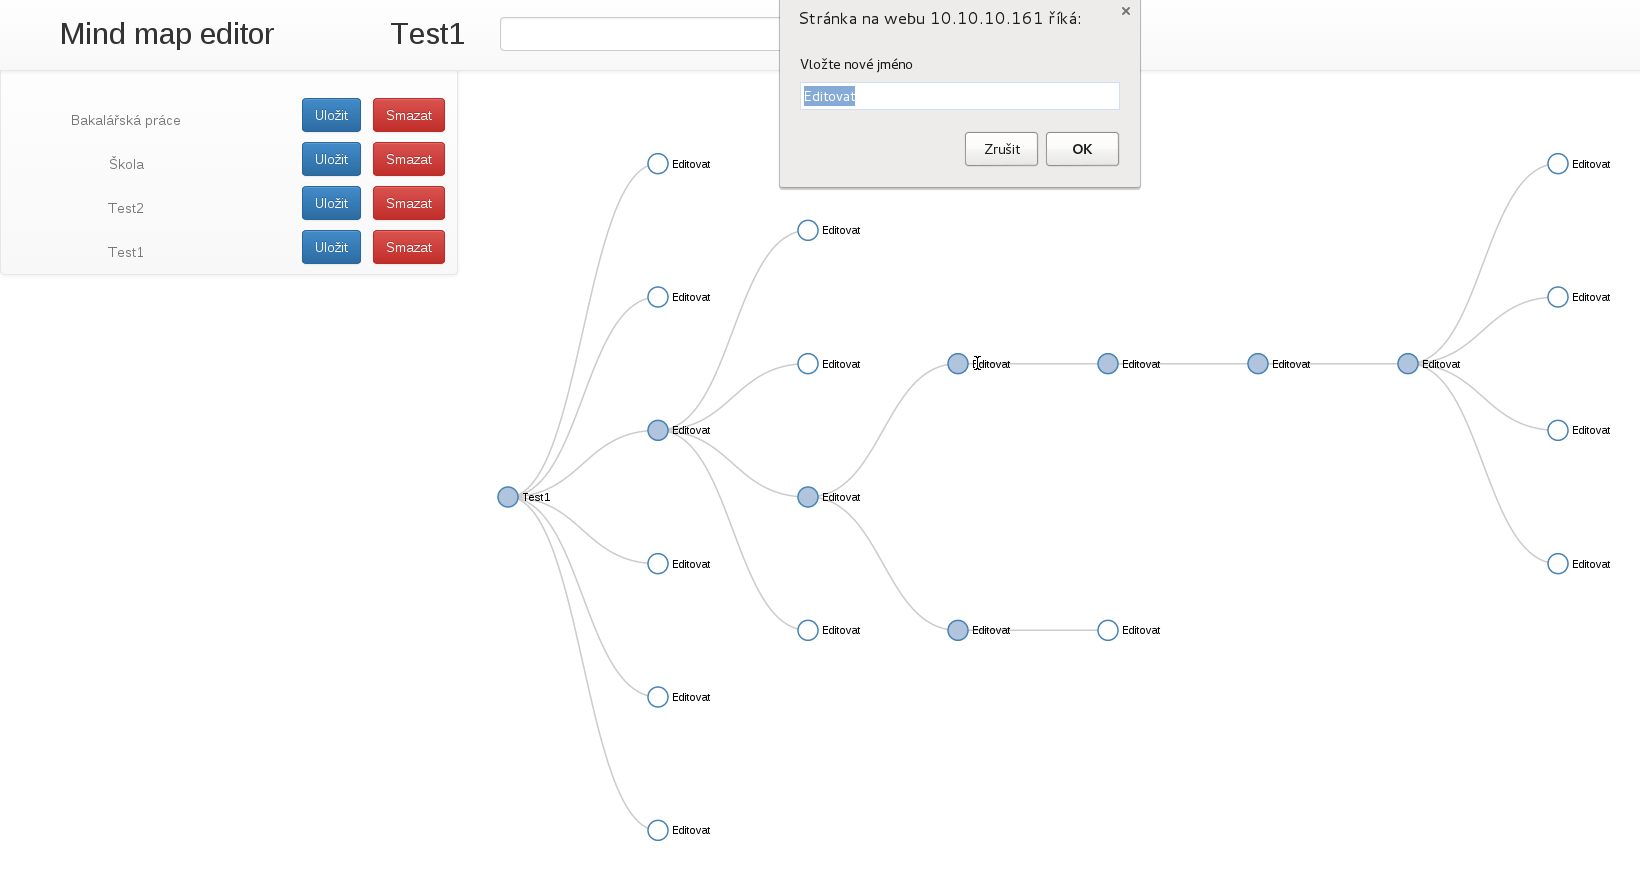
\includegraphics[width	=1\textwidth]{obrazky/mindmap3}
\par\end{centering}
\caption{Webová aplikace - akce - editace\label{fig:midnmap3}}
\end{figure}

Parametr \emph{auto-redeploy} mluví sám za sebe.

Jak bylo řečeno v \ref{sub:hybrid} Vert.x instance má dvě sady vláken. Parametrem \emph{worker} v deskriptoru modulu, lze říci Vert.x jádru aby spustil modul v \emph{background worker poolu}. 

Spuštění modulu programově v jazyce Java
\begin{lstlisting}
container.deployModule("io.vertx~mod-mailer~2.0.0-beta1", JSONconfig);
\end{lstlisting}

Spuštění modulu z příkazové řádky
\begin{lstlisting}
vertx runmod com.mycompany~my-mod~1.0 -conf config.json
\end{lstlisting}

moduly vice jazyku

\section{Nasazení}

deploy + scaling

\subsection{Server}

ubuntu

\subsection{Java}

java

\subsection{Vert.x}

vert.x

\subsection{MongoDB}

mongodb

\section{Škálování a vysoká dostupnost}\label{sub:Scaling}

možnosti škálování a HA

\subsection{Počet Verticlů}
verticle count

\subsection{Interakce s Vert.x}\label{sub:interaction}

Díky modulu CrasHub Shell\footnote{https://github.com/crashub/mod-shell} se lze protokolem SSH\footnote{Secure Shell} přihlásit přímo do Vert.x. Modul pak nabízí možnost interakce s jednotlivými komponentami samotného Vert.x. Lze například posílat zprávy přes Event Bus nebo nasazovat nové moduly za běhu celé aplikace. Samotný modul pak nabízí jednoduchou možnost přidání vlastním příkazů. Na obrázku je pak vidět přehledová obrazovka. Na obrazovce je seznam všech vláken, celkové velikost zásobníku či verze použité Javy. 

\begin{figure}
\begin{centering}
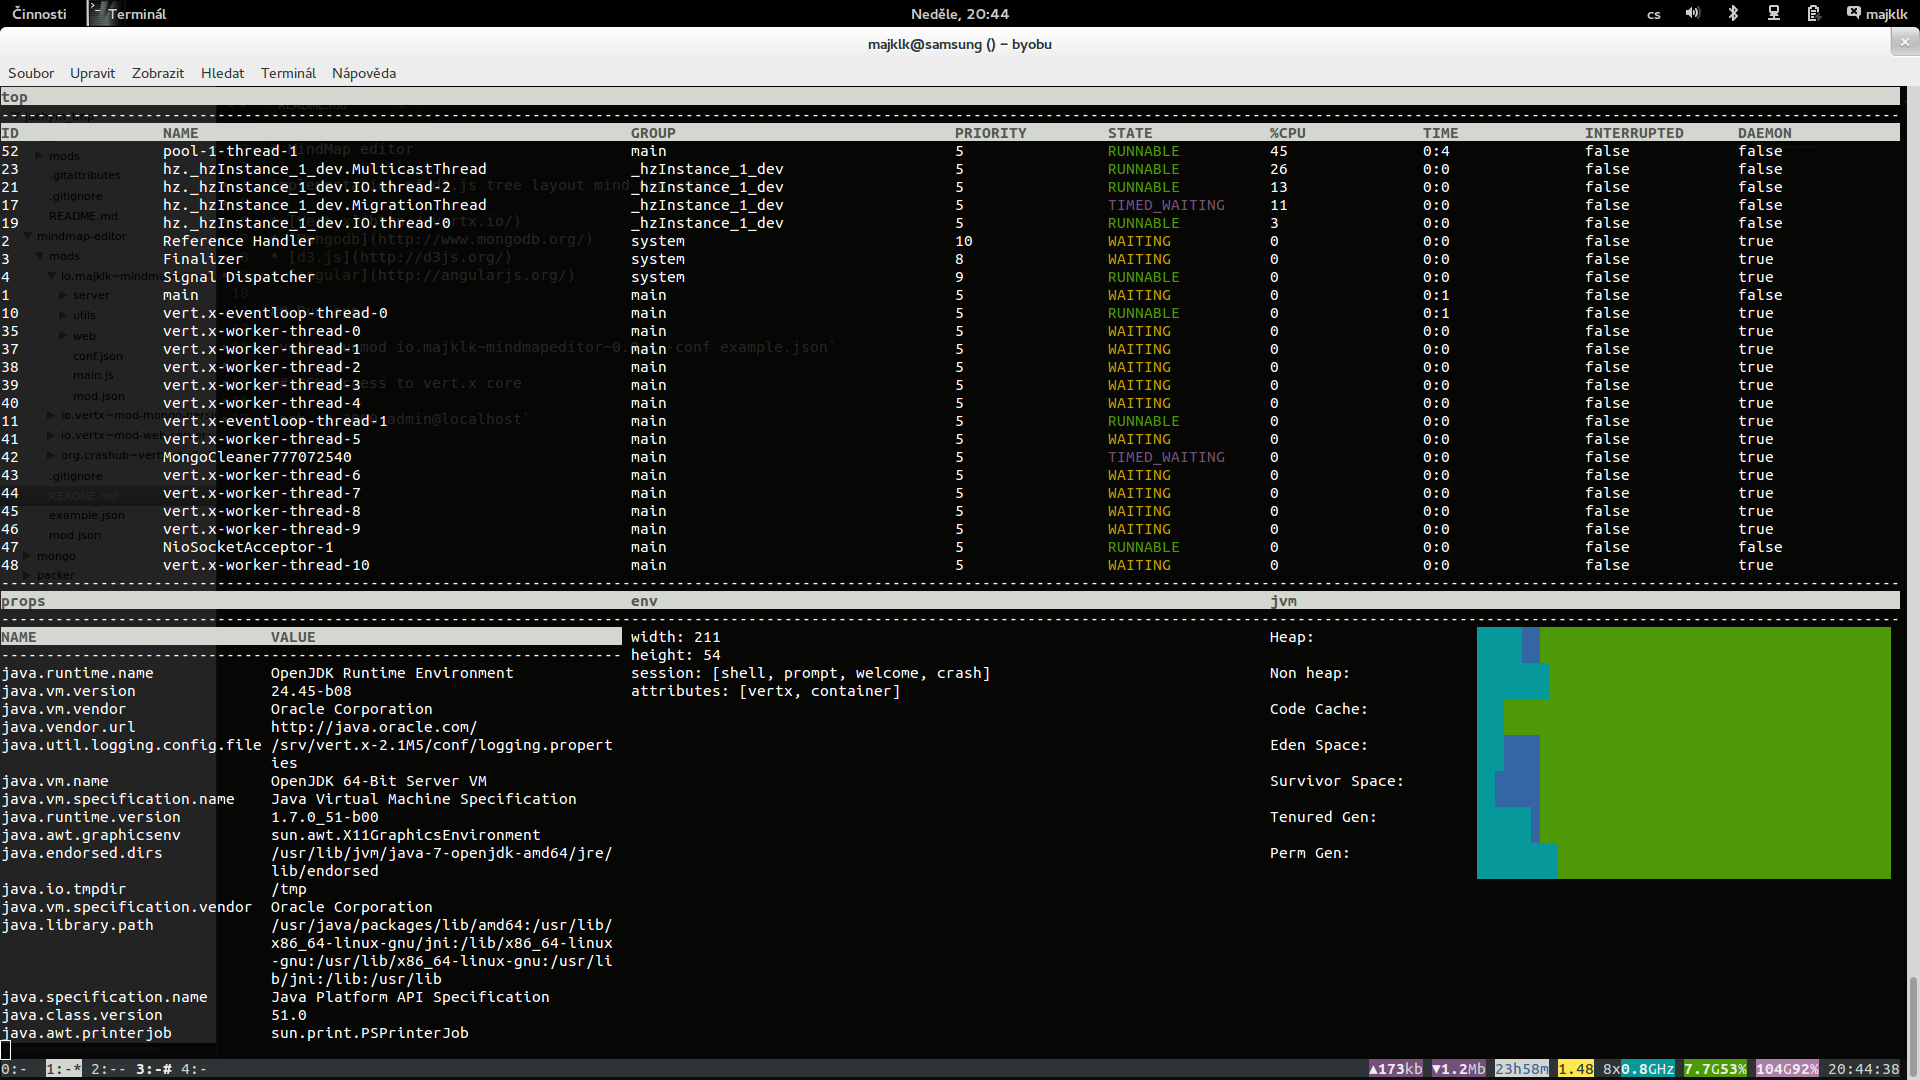
\includegraphics[scale=0.21]{obrazky/real_interaction}
\par\end{centering}
\caption{Modul CrasHub Shell\label{fig:real_interaction}}
\end{figure}

\subsection{Vert.x v clusteru}\label{sub:praktCluster}

Pro zajištění bezpečnosti databázového serveru, kde běží také služba pro vzdálený přístup k Vert.x instanci bude aplikace nasazena v clusteru. Webový server(HTTP Server) na obrázku \ref{fig:architecture_real} je připojen do dvou sítí.

\begin{description}
\item[Internet] pouze webový server
\item[Síť clusteru] všechny servery
\end{description}

Pro maximální bezpečnost budou na webovém serveru otevřeny pouze porty 80 a 443. Na druhém serveru pak poběží samotná databáze a druhá část aplikace, která v sobě bude zahrnovat modul zajištující komunikaci s databází a modul pro vzdálenou správu Vert.x instancí, který byl představen v kapitole \ref{sub:interaction}.

\begin{figure}
\begin{centering}
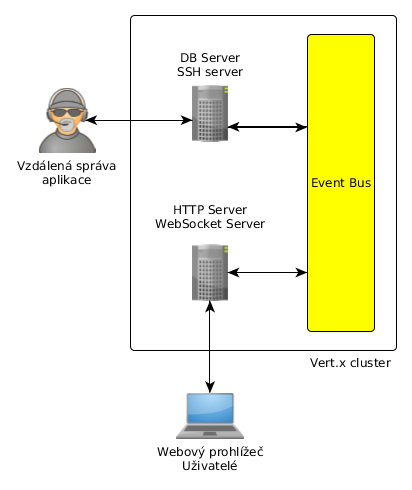
\includegraphics[scale=0.5]{obrazky/architecture_real}
\par\end{centering}
\caption{Architektura nasazené aplikace\label{fig:architecture_real}}
\end{figure}

\subsection{Vysoká dostupnost}

Pro zajištění vysoké dostupnosti klíčových prvků aplikace, je potřeba upravit architekturu clusteru. Před webový server je postavená HA proxy\footnote{služba zajištující vyrovnávání zatížení}, která při úpadku jednoho z webových serverů přesměruje komunikaci na server druhý. Vert.x cluster je pak rozdělený na dvě HA skupiny(obr.\ref{fig:architecture_ideal}), které se liší svým zaměřením. První dva servery slouží jako webové a jsou napojeny na HA proxy. Další dva pak slouží pro komunikaci s databází, která na nich ležet nemusí.

\begin{figure}
\begin{centering}
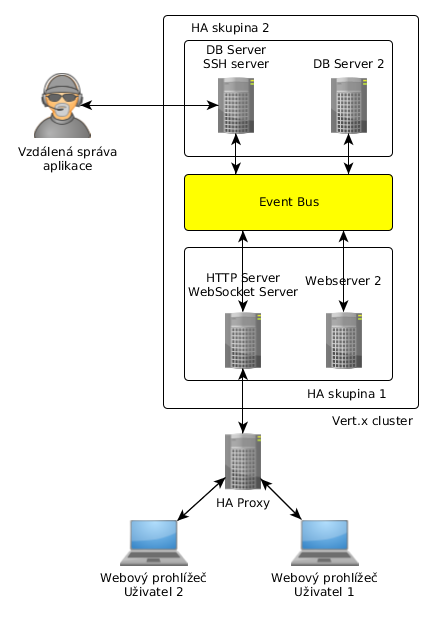
\includegraphics[scale=0.5]{obrazky/architecture_ideal}
\par\end{centering}
\caption{Ideální architekutra nasazení aplikace\label{fig:architecture_ideal}}
\end{figure}
